\documentclass[ 12pt,a4paper,twocolumn,fleqn]{article}
\usepackage{graphicx}
\usepackage[a4paper,top=20mm, bottom=30mm, left=10mm, right=25mm]{geometry}
\usepackage{fancyhdr}
\usepackage{hyperref}
\usepackage{listings}
\usepackage[]{algorithm2e}
\usepackage{color}
\usepackage{fancybox}
\thisfancypage{%
  \setlength{\fboxsep}{20pt}\doublebox}{}
\pagestyle{fancy}
\usepackage{lineno}
\usepackage{xtab,booktabs}
\usepackage{setspace}
\usepackage{amsmath}
\usepackage{xcolor}
\usepackage[compact]{titlesec}
\titlespacing{\section}{0pt}{*0}{*0}
\titlespacing{\subsection}{0pt}{*0}{*0}
\titlespacing{\subsubsection}{0pt}{*0}{*0}
\setlength\columnsep{25pt}
\makeatletter
\g@addto@macro{\normalsize}{%
\setlength{\abovedisplayskip}{0pt}
\setlength{\abovedisplayshortskip}{0pt}
\setlength{\belowdisplayskip}{0pt}
\setlength{\belowdisplayshortskip}{0pt}}
\makeatother
\mathindent=0.0pt
\usepackage{float}
\renewcommand{\baselinestretch}{1.5}
\begin{document}
\lhead{Project Title Here}
\chead{}
\rhead{Team Members, Batch Number here}
\onecolumn
\begin{center}
\text{A Project Report On} \\
\smallskip
\textcolor{red}{\LARGE{THE PROJECT TITLE GOES HERE}} \\
\large{Submitted in partial fulfillment of the requirement for the $8^{th}$ semester}
\large{\textbf{Bachelor of Engineering}} \\
\large{in} \\
\large{Computer Science and Engineering} \\
\textcolor{blue}{\LARGE{DAYANANDA SAGAR COLLEGE OF ENGINEERING}} \\
\footnotesize{(An Autonomous Institute affiliated to VTU, Belagavi, Approved by AICTE \& ISO 9001:2008 Certified)} \\
\footnotesize{Accredited by National Assessment \& Accreditation Council (NAAC) with ‘A’ grade}  \\
\footnotesize{Shavige Malleshwara Hills, Kumaraswamy Layout, Bengaluru-560078} \\

\includegraphics[scale=0.4]{media/DSCE-min.png} \\
\textit{Submitted By} \\
\textbf{John Doe \space 1DS17CS001} \\
\textbf{Mary Sue \space 1DS17CS002} \\
\textbf{Marty Sue \space 1DS17CS003} \\
\textbf{Mark Twain \space 1DS17CS004} \\
\textit{Under the guidance of} \\
\textbf{Dr. Firstname Lastname}
\hfill
\textbf{Dr. Secondname Lastname} \\
\text{Professor, CSE , DSCE}
\hfill
\text{Asst Professor, CSE , DSCE} \\
\Large{\textbf{2020 - 2021}} \\
\textcolor{blue}{\Large{Department of Computer Science and Engineering}} \\
\textcolor{blue}{\Large{DAYANANDA SAGAR COLLEGE OF ENGINEERING}} \\
\textcolor{blue}{\Large{Bangalore - 560078}} \\
\end{center}
\newpage
  \pagestyle{fancy}
\thisfancypage{%
  \setlength{\fboxsep}{20pt}\doublebox}{}
\begin{center}
\textcolor{red}{\LARGE{VISVESVARAYA TECHNOLOGICAL UNIVERSITY}} \\
\textcolor{red}{\LARGE{Dayananda Sagar College of Engineering}} \\
\footnotesize{(An Autonomous Institute affiliated to VTU, Belagavi, Approved by AICTE \& ISO 9001:2008 Certified)} \\
\footnotesize{Accredited by National Assessment \& Accreditation Council (NAAC) with ‘A’ grade}  \\
\footnotesize{Shavige Malleshwara Hills, Kumaraswamy Layout, Bengaluru-560078} \\
\begin{flushleft}
\textcolor{blue}{\LARGE{\textbf{Department of Computer Science \& Engineering}}} \\
\end{flushleft}

\includegraphics[scale=0.4]{media/DSCE-min.png} \\
\Large{\underline{\textbf{CERTIFICATE}}} \\
  \end{center}
\normalsize
This is to certify that the project entitled \textbf{[Project Title Goes Here]} is a bonafide work carried out by \textbf{John Doe [1DS17CS001]}, \textbf{Mary Sue [1DS17CS002], Marty Sue [1DS17CS003]} and \textbf{Mark Twain [1DS17CS004]} in partial fulfillment of 8th semester, Bachelor of Engineering in Computer Science and Engineering under Visvesvaraya Technological University, Belgaum during the year 2020-21. \\
\\
\textbf{Dr. Firstname Lastname}
\hfill
\textbf{Dr. Ramesh Babu D R}
\hfill
\textbf{Dr. C P S Prakash} \\
\text{(Internal Guide)}
\hfill
\text{Vice Principal \& HOD}
\hfill
\text{Principal} \\
\text{Asst Prof. CSE, DSCE} 
\hfill
\text{CSE, DSCE}
\hfill
\text{DSCE} \\
\\
\text{Signature:...........}
\hfill
\text{Signature:...........}
\hfill
\text{Signature:...........} \\
\\
\\
\text{Name of the Examiners:}
\hfill
\text{Signature with date:} \\
\text{1...........................}
\hfill{.............................} \\
\text{2.............................} 
\hfill{............................} \\
\newpage
  \pagestyle{fancy}
\thisfancypage{%
  \setlength{\fboxsep}{20pt}\doublebox}{}
\begin{center}
\LARGE{{\underline{Acknowledgement}}} \\
\end{center}
\normalsize
We are pleased to have successfully completed the project \textbf{[Project Title Goes Here]}. We thoroughly enjoyed the process of working on this project and gained a lot of knowledge doing so.
\\
\hfill
\\
We would like to take this opportunity to express our gratitude to \textbf{Dr. C P S Prakash}, Principal of DSCE, for permitting us to utilize all the necessary facilities of the institution.
\\
\hfill
\\
We also thank our respected Vice Principal, HOD of Computer Science \& Engineering, DSCE, Bangalore,\textbf{ Dr. Ramesh Babu D R}, for his support and encouragement throughout the process.
\\
\hfill
\\
We are immensely grateful to our respected and learned guide, \textbf{[Guide Name]}, Professor CSE, DSCE and our co-guide \textbf{[Name]}, Assistant professor, CSE, DSCE for their valuable help and guidance. We are indebted to them for their invaluable guidance throughout the process and their useful inputs at all stages of the process.
\\
\hfill
\\
We also thank all the faculty and support staff of Department of Computer Science, DSCE. Without their support over the years, this work would not have been possible.
\\
\hfill
\\
Lastly, we would like to express our deep appreciation towards our classmates and our family for providing us with constant moral support and encouragement. They have stood by us in the most difficult of times.
\\
\hfill
\\
\begin{flushright}
\textbf{John Doe \space 1DS17CS001} \\
\textbf{Mary Sue \space 1DS17CS002} \\
\textbf{Marty Sue \space 1DS17CS003} \\
\textbf{Mark Twain \space 1DS17CS004} \\
\end{flushright}
\newpage
  \pagestyle{fancy}
\thisfancypage{%
  \setlength{\fboxsep}{20pt}\doublebox}{}
\setstretch{1.5}
\twocolumn[
\begin{@twocolumnfalse}
\title {[Project Title Goes Here]}
\author{John Doe, Mary Sue, Marty Sue, Mark Twain}
\maketitle
\begin{abstract}
This is a sample abstract. It should consist of a single paragraph of no more than 250 - 300 words. Describe the background, goals and methodology of your project in brief here. Use full, short sentences instead of punctuating your sentences with multiple commas. The Abstract typically does not include blank lines between the paragraphs, but you may include them. Do not include any images here. What follows is random text to fill up the space to show you what the desired length (including these words) looks like.  Lorem ipsum dolor sit amet, consectetur adipiscing elit, sed do eiusmod tempor incididunt ut labore et dolore magna aliqua. Ut enim ad minim veniam, quis nostrud exercitation ullamco laboris nisi ut aliquip ex ea commodo consequat. Duis aute irure dolor in reprehenderit in voluptate velit esse cillum dolore eu fugiat nulla pariatur. Excepteur sint occaecat cupidatat non proident, sunt in culpa qui officia deserunt mollit anim id est laborum. Sed ut perspiciatis unde omnis iste natus error sit voluptatem accusantium doloremque laudantium, totam rem aperiam, eaque ipsa quae ab illo inventore veritatis et quasi architecto beatae vitae dicta sunt explicabo. Nemo enim ipsam voluptatem quia voluptas sit aspernatur aut odit aut fugit, sed quia consequuntur magni dolores eos qui ratione voluptatem sequi nesciunt. Neque porro quisquam est, qui dolorem ipsum quia dolor sit amet, consectetur, adipisci velit, sed quia non numquam eius modi tempora incidunt ut labore et dolore magnam aliquam quaerat voluptatem. Ut enim ad minima veniam, quis nostrum exercitationem ullam corporis suscipit laboriosam, nisi ut aliquid ex ea commodi consequatur? Quis autem vel eum iure reprehenderit qui in ea voluptate velit esse quam nihil molestiae consequatur, vel illum qui dolorem eum fugiat quo voluptas nulla pariatur. \textbf{(286 words)}.
\end{abstract}
\end{@twocolumnfalse}]
\linenumbers
\modulolinenumbers[5]
\onecolumn
\newpage
  \pagestyle{fancy}
\thisfancypage{%
  \setlength{\fboxsep}{20pt}\doublebox}{}
\tableofcontents
\newpage
  \pagestyle{fancy}
\thisfancypage{%
  \setlength{\fboxsep}{20pt}\doublebox}{}
\part{Overview}
Welcome to the main body of the report. As you can see we have used the part tag above to label the first part of our report, called the overview. We have done this so that \LaTeX{} can automatically number our document. There are multiple tiers to this numbering, such as sections, subsections, subsubsections and paragraphs. You can also use chapters, but for that at the top of the document you must enable report instead of article. I think 4 levels of nesting is enough. \LaTeX{} also uses the information you have given it to populate the table of contents (Index). So please use the appropriate tags instead of manually changing the font, it will make your document easier to edit, maintain and will also give you a neatly formatted index.
\section{Sample Section}
This is a section. I have used the section tab which you can view in the source file.
\subsection{Sample Subsection}
This is a sample subsection. This uses the subsection tab which you can view in the source file. This also numbers the subsection with a decimal with the section number as its root. To start a new section just use the section tab again!
\subsubsection{Sample Subsubsection}
This is a sample subsubsection. Note that the numbering is a subset of the subsection. This also indents the index to the right. You may also notice that the size of the titles decreases as you go lower.
\section{text formatting}
\LaTeX{} includes some default text sizes. These are labelled: \\
\huge{huge} \\
\LARGE{LARGE} \\
\Large{Large} \\
\large{large} \\
\normalsize{normalsize} \\
\small{small} \\
\footnotesize{footnotesize} \\
\scriptsize{scriptsize}
\newpage
  \pagestyle{fancy}
\thisfancypage{%
  \setlength{\fboxsep}{20pt}\doublebox}{}
\normalsize
\subsection{Bold, Italics, Underline and mathmode}
You can use the text{} tag for normal text. If you are typing paragraphs, it is best to not use any markup as this may cause overflow errors. the textbf tag will give you \textbf{bold text}. You can also use Texmaker's B button on the left editing pane. \\
You can use textit tag for italics. This will \textit{italicize the text}. You can also use Texmaker's i button on the left editing pane. \\
You can use the underline tag for underline. This will \underline{underline the text}. \\
Rendering beautiful equations is one of the features of \LaTeX{}. You can represent Greek and other symbols easily by using the backslash with the symbol name. However to do this you must first enable mathmode. You can do this by using Dollar symbols to encase the mathematical symbols. I use flalign to align my equations properly. Given below are some samples:
\begin{flalign} \begin{aligned} Stall \, velocity \; V_{stall} = \sqrt{\frac{2W}{\rho S (C_{L})_{max}}} \end{aligned} \end{flalign}
\begin{flalign}
\begin{split}
Take off distance \,Sg= \\
\frac{1.21(W/S)}{g \rho_{ \infty} C_{Lmax}(T-D/W)-\mu_{r}(1-(L/W))]_{0.7VTO}} \\+
1.1N\sqrt{\frac{2W}{\rho S C_{Lmax}}}
\end{split}
\end{flalign} \\
You can see that \LaTeX{} also numbers our equations for us!
\subsection{Coloured Text}
We can use the textcolour tag to color our text (color is spelt with an american spelling). You can also nest the text styles and sizes mentioned above into the colour tags to produce custom text with different font styles, sizes and colours. Given below are some samples: \\
\hfill
\\
\textcolor{red}{\LARGE{Large red coloured text}} \\
\textcolor{blue}{\normalsize{Normal blue coloured text}} \\
\textcolor{green}{\normalsize{\textbf{Bold green coloured text}}} \\
\textcolor{yellow}{\normalsize{\textit{Italicized yellow coloured text}}}
\newpage
  \pagestyle{fancy}
\thisfancypage{%
  \setlength{\fboxsep}{20pt}\doublebox}{}
\twocolumn
\section{Two Column}
If you want your report to have the look of a research paper, you can use the twocolumn tag. If you want to switch out of two columns, you can just use the onecolumn tag again. The empty space between the columns is determined by the columnsep parameter, which is at the head of the file. \\
\\
You can use the multicols package for 2 or even 3 column layouts and switch dynamically between them on the same page. This however may cause formatting issues and is generally not recommended. If you need to switch to two columns, use a new page to avoid formatting issues. The rest of this page is random text to show you how a two column layout looks.
\\
Lorem ipsum dolor sit amet, consectetur adipiscing elit, sed do eiusmod tempor incididunt ut labore et dolore magna aliqua. Ut enim ad minim veniam, quis nostrud exercitation ullamco laboris nisi ut aliquip ex ea commodo consequat. Duis aute irure dolor in reprehenderit in voluptate velit esse cillum dolore eu fugiat nulla pariatur. Excepteur sint occaecat cupidatat non proident, sunt in culpa qui officia deserunt mollit anim id est laborum.
\\
Sed ut perspiciatis unde omnis iste natus error sit voluptatem accusantium doloremque laudantium, totam rem aperiam, eaque ipsa quae ab illo inventore veritatis et quasi architecto beatae vitae dicta sunt explicabo. Nemo enim ipsam voluptatem quia voluptas sit aspernatur aut odit aut fugit, sed quia consequuntur magni dolores eos qui ratione voluptatem sequi nesciunt. Neque porro quisquam est, qui dolorem ipsum quia dolor sit amet, consectetur, adipisci velit, sed quia non numquam eius modi tempora incidunt ut labore et dolore magnam aliquam quaerat voluptatem. Ut enim ad minima veniam, quis nostrum exercitationem ullam corporis suscipit laboriosam, nisi ut aliquid ex ea commodi consequatur? Quis autem vel eum iure reprehenderit qui in ea voluptate velit esse quam nihil molestiae consequatur, vel illum qui dolorem eum fugiat quo voluptas nulla pariatur?
At vero eos et accusamus et iusto odio dignissimos ducimus qui blanditiis praesentium voluptatum deleniti atque corrupti quos dolores et quas molestias excepturi sint occaecati cupiditate non provident, similique sunt in culpa qui officia deserunt mollitia animi, id est laborum et dolorum fuga. Et harum quidem rerum facilis est et expedita distinctio. Nam libero tempore, cum soluta nobis est eligendi optio cumque nihil impedit quo minus id quod maxime placeat facere possimus, omnis voluptas assumenda est, omnis dolor repellendus. \\
\\
This is the end of two column view.
\onecolumn
\newpage
  \pagestyle{fancy}
\thisfancypage{%
  \setlength{\fboxsep}{20pt}\doublebox}{}
\subsection{Hyperlinks}
\LaTeX{} provides us with Hyperlinks via the Hyperref package. You can use the href tag to link to a URL and name it something. The url tag can be used to link a URL without an alias. The mailto option can be used when referring to an email ID so that the mail client opens up directly when clicked. Latex generated PDFs also show a blue box around links. Examples below: \\
Link with alias: \href{https://dsce.edu.in/}{DSCE - Homepage} \\
Link without alias: \url{https://dsce.edu.in/} \\
My email address is: \href{mailto:ashutosh@gnu.org}{ashutosh@gnu.org} \\
Combine color with href: \textcolor{blue}{\href{https://dsce.edu.in/}{DSCE - Homepage}} \\
\section{Code and Algorithms}
\subsection{Code}
\LaTeX{} provides us with several packages to handle code. Some of these include verbatim and listings. Listings is far more powerful and as usual, it has to be declared in the header with the usepackage along with colour. Later we define lstset (given in the source file). We define the language and what colours we want for the keywords, numbers, comments et al. An example output is given below: \\
\definecolor{dkgreen}{rgb}{0,0.6,0}
\definecolor{gray}{rgb}{0.5,0.5,0.5}
\definecolor{mauve}{rgb}{0.58,0,0.82}

\lstset{frame=tb,
  language=Java,
  aboveskip=3mm,
  belowskip=3mm,
  showstringspaces=false,
  columns=flexible,
  basicstyle={\small\ttfamily},
  numbers=none,
  numberstyle=\tiny\color{gray},
  keywordstyle=\color{blue},
  commentstyle=\color{dkgreen},
  stringstyle=\color{mauve},
  breaklines=true,
  breakatwhitespace=true,
  tabsize=3
}
\begin{lstlisting}
// Hello.java
import javax.swing.JApplet;
import java.awt.Graphics;

public class Hello extends JApplet {
    public void paintComponent(Graphics g) {
        g.drawString("Hello, world!", 65, 95);
    }    
}
\end{lstlisting}
\newpage
  \pagestyle{fancy}
\thisfancypage{%
  \setlength{\fboxsep}{20pt}\doublebox}{}
\subsection{Algorithms}
Algorithms or Pseudocode can be written using Algorithm2E or Algorithm (deprecated) or Algorithmx packages. Here is an example using Algorithm2e. The package must be included in the document preamble.
\begin{algorithm}[H]
 \KwData{this text}
 \KwResult{how to write algorithm with \LaTeX2e }
 initialization\;
 \While{not at end of this document}{
  read current\;
  \eIf{understand}{
   go to next section\;
   current section becomes this one\;
   }{
   go back to the beginning of current section\;
  }
 }
 \caption{How to write algorithms}
\end{algorithm}
\section{Tables}
\LaTeX{} provides several packages for tables. It is easy to draw and modify tables with any number of rows and columns. The table will automatically flow to the next page incase it does not fit in one page. You can use the Xtabs or tabular package to handle many different types of tables. Given below is a sample:
\begin{table}[H]
\centering
\footnotesize
\begin{tabular}{|p{2cm}| p{2cm} |p{2cm}|p{2cm}|p{2cm}|}
\hline
Comp & Ult Load (N) & LA (N) & FoS & MoS\\
\hline\hline
Wing & 10 & 12 & 13 & 43\\
Fuselage & 45.14 & 66.67 & 1.4 & 47\\
Boom & 978 & 3.42 & 286 & 186\\
Landing gear & 490.32 & 294 & 13.67& 03.67\\
\hline
\end{tabular}
\caption{Critical Margins Table}
\label{table:10}
FoS = Factor of Safety \\
MoS = Margin of Safety \\
\end{table}
The width of the rows and other properties can be edited on the first line begin tabular (see source). Try to avoid multiple table packages together as this may lead to errors.
\newpage
  \pagestyle{fancy}
\thisfancypage{%
  \setlength{\fboxsep}{20pt}\doublebox}{}
\section{Images}
\LaTeX{} provides the graphicx package to include images. There are special packages to handle text warping, but using Minipages is a convenient way of handling images. Sample given below: \\
\hfill
\\
\begin{figure}[H]
\begin{minipage}{0.5\textwidth}
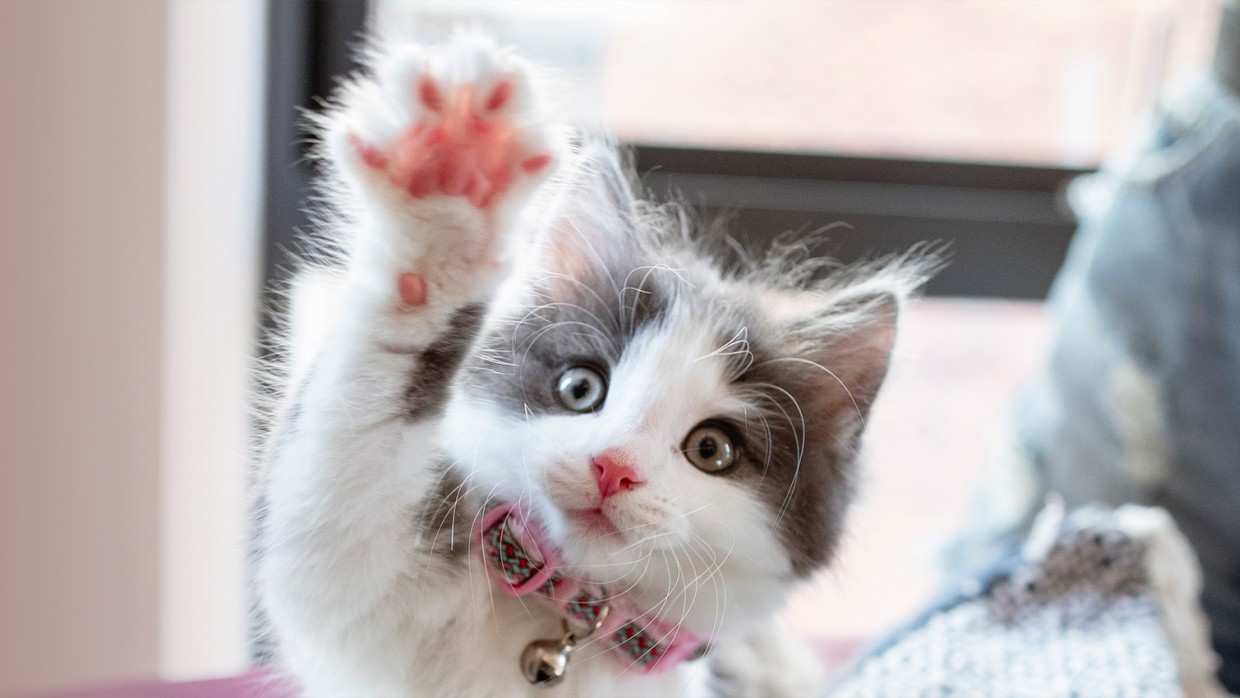
\includegraphics[width=7cm,height=5cm]{media/Kitten}
\centering
\caption{Hello, I am a cat}
\end{minipage}
\begin{minipage}
{.5\textwidth}
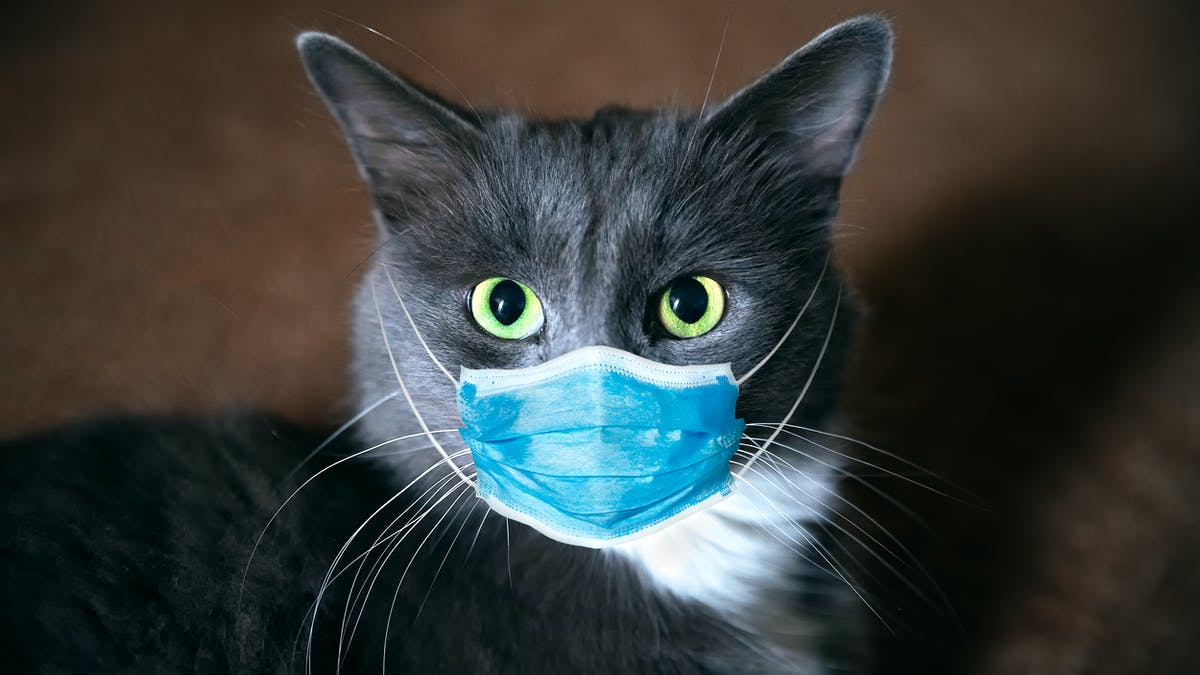
\includegraphics[width=7cm,height=5cm]{media/Kitten2}
\centering
\caption{Another cat}
\end{minipage}
\end{figure}
Be sure to check the hyperlinks to the figures. Change the file names to something you can easily remember to avoid getting confused. Make sure all the begin and end tabs are proper, else the images will not render. You can also use scale instead of absolute values in centimeters or millimeters.
\section{References}

To include References the right way (using Biblatex), search for a Bibtex generator on Google, and feed its output to a seperate Bibtex (Bib) file. Then we simply reference it in our main file and you will get the citations neatly ordered. If you want a quicker (improper hack), then just paste the results of the citation generator. \\
$[1]$ Figure 2f from: Irimia R, Gottschling M (2016) Taxonomic revision of Rochefortia Sw. (Ehretiaceae, Boraginales). Biodiversity Data Journal 4:e7720 
\\
$[2]$ BRANDON, J. 2007. Similarity of temporal query logs. Doctoral dissertation. University of California, Los Angeles. \\

Please note that the citation formats for different documents (articles, reports, dissertations,papers, conference proceedings) and organisations (ACM, IEEE) are different. Use a consistent style.
\end{document}